\newpage
\section{Detaillierte Projektbeschreibung}

	\subsection{Modulare Eurorack Synthesizer}
	
	In der modernen elektronischen Musikproduktion erfreut sich die Modularität von Synthesizern wieder großer Beliebtheit. 
	Die Methoden, verschiedene Module von unterschiedlichen Herstellern miteinander zu kombinieren, erleben ein Revival. \cite{ferguson2015interview}
	Wo einst die Reise der elektronischen Musik begann, werden diese Ansätze erneut aufgegriffen.
	
	In den 1950er Jahren erzeugten die Pioniere der elektronischen Musik mit Labor- und Testequipment neue Klänge. 
	Signalgeneratoren, Filter und anderes technisches Gerät aus den Ingenieurlabors wurden funktional zu Musikinstrumenten umgewandelt – die elektronische Musik war geboren. \cite{holmes2002electronic}
	
	In den 1990er Jahren, durch die bessere Zugänglichkeit und günstigeren Kosten von Chips und Halbleitern, fand dieses Mindset den Weg zu den Consumer-Musikproduzenten - Dieter Doepfer entwickelte den Eurorack-Standard für modulare Synthesizer. \cite{eurorack-standard}
	
	Die Module sind in 3U-Höhe (etwa 133,4 mm) und variabler Breite in HP (horizontal pitch) erhältlich, wobei 1 HP etwa 5,08 mm entspricht. Diese Maße basieren auf dem 19"-Rack-Standard, der in Computertechnik und Audio Equipment weit verbreitet ist. Die Module werden in Racks oder Cases montiert, die mit Schienen ausgestattet sind, um eine flexible und modulare Konfiguration zu ermöglichen. \cite{iec60297-3-108:2014}
	
	
	\begin{figure}[h!]
		\centering
		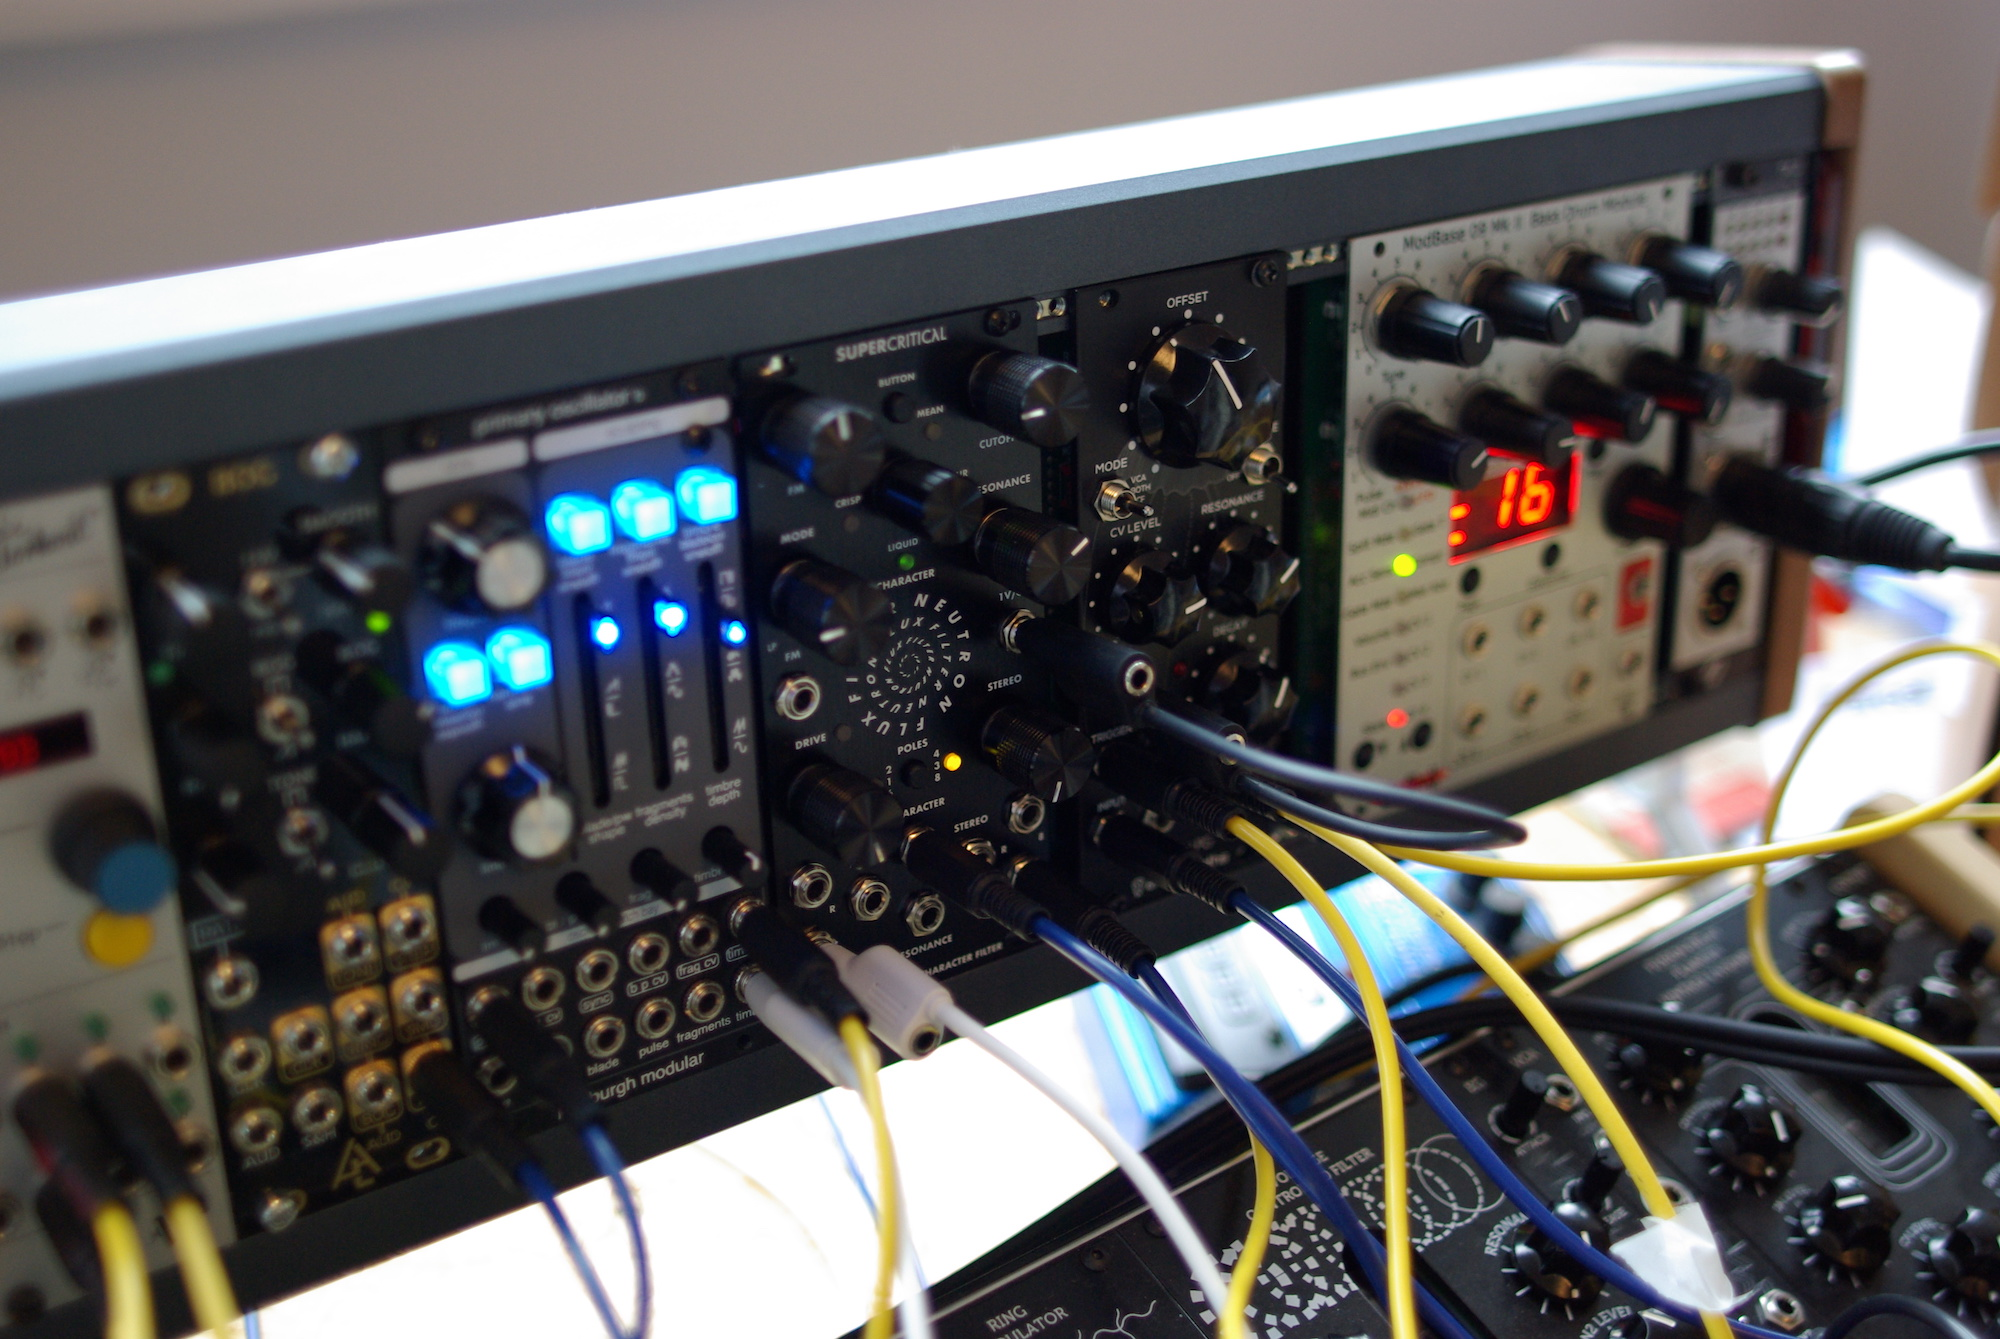
\includegraphics[width=0.5\textwidth]{images/02_detaillierte-projektbeschr/eurorack-patched}
		\caption{Gepatchtes Eurorack 3U Rack (einreihig)}
		\label{fig:eurorack-patched}
	\end{figure}
	
	Elektrisch werden Eurorack-Module über eine gemeinsame Stromversorgung betrieben, die typischerweise +12V, -12V und manchmal +5V bereitstellt. Module werden über 10-polige oder 16-polige Flachbandkabel an eine Stromverteilungsplatine (Bus Board) angeschlossen. Die wichtigsten elektrischen Verbindungen umfassen +12V, -12V und GND, wobei der 16-polige Anschluss zusätzlich +5V und weitere Signale unterstützen kann. \cite{eurorack-standard}
	
	Für die Signalübertragung nutzen Eurorack-Module 3,5 mm Monoklinkenstecker, um die Module miteinander zu ``verpatchen``. Über diese Kabel werden Audiosignale (typischerweise ±5V), Steuersignale (CV) und Triggersignale (0V bis +5V) zwischen den Modulen übertragen.
	
	Audiosignale, Steuersignale und Triggersignale werden also mit denselben Buchsen und Kabeln verbunden.
	Dies eröffnet enorme Möglichkeiten, die Klangpalette zu erweitern. So können beispielsweise Audiosignale zur Steuerung der Parameter eines Moduls verwendet werden, was kreative und innovative Patches ermöglicht.
	
	Mit der Eurorack Revolution haben sich modulare Synthesizer auch technisch weiterentwickelt. 
	Es wird vermehrt auf digitale Module gesetzt. 
	Die Zeit der Analog-Puristen ist vorbei; alle Möglichkeiten der digitalen Signalverarbeitung werden genutzt, um innovative Module zu entwerfen, die neue Methoden und Ideen in das eigene Rack bringen.
	
	Eine Unterkategorie der digitalen Module bilden die Audiosampler. Diese Module nehmen digitale Aufnahmen (Samples) von Klängen oder Musikstücken auf, speichern und spielen sie ab. Die Samples können durch verschiedene Trigger aktiviert und in unterschiedlichen Tonhöhen und Geschwindigkeiten abgespielt werden. 
	Audiosampler ermöglichen es Musikern, realistische Klänge von Instrumenten, Stimmen oder Umweltgeräuschen in ihre Musik zu integrieren und kreativ zu manipulieren.
	
	\subsection{Das Konzept}
	
	Es gibt durchaus Audiosampler mit ergonomischer Steuerung, großen hochauflösenden Displays und zahlreichen Knöpfen, um diese komplexen Audiomaschinen angenehm zu steuern. 
	Beispiele hierfür sind die legendäre MPC von AKAI oder der Octatrack von Elektron. 
	
	Die Hardware dieser Geräte sind jedoch aufgrund ihrer Bedienelemente und der damit einhergehenden Ergonomie so groß, dass sie unmöglich in ein Eurorack unterzubringen sind.
	
	\begin{wrapfigure}{r}{0.4\textwidth} % Increase the width of the figure environment
		\vspace{-20pt + 0.02\textwidth}
		\hspace{0.02\textwidth} % Add horizontal space
		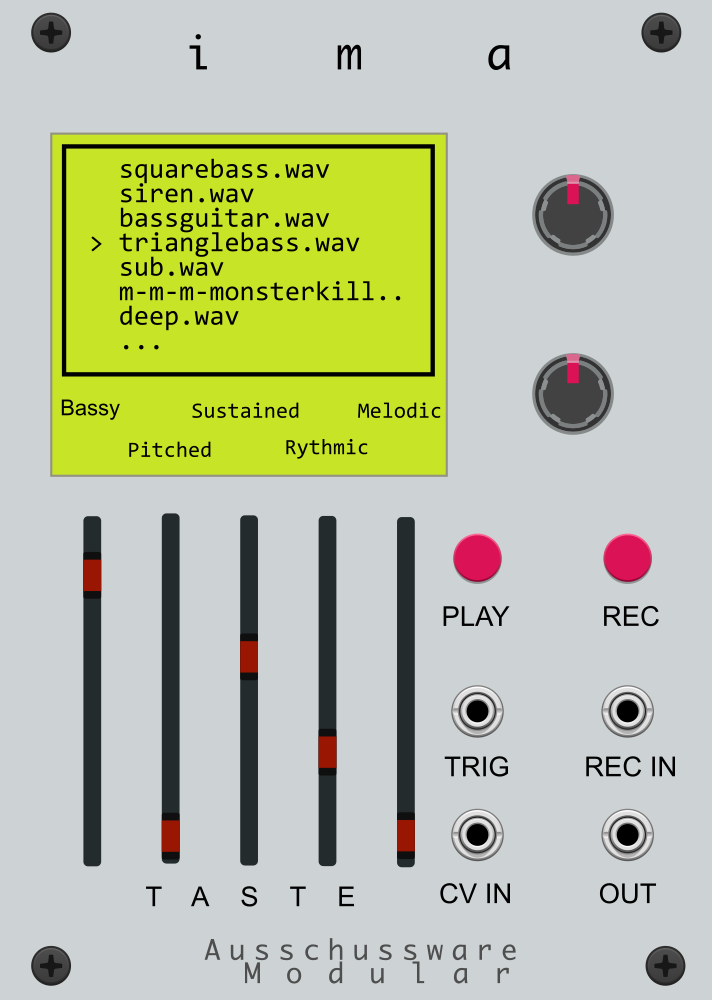
\includegraphics[width=0.38\textwidth]{images/02_detaillierte-projektbeschr/ima_mockup.png} % Keep the image size the same
		\caption{Panel Design Mockup }
		\label{fig:panel_mockup}
		\vspace{-20pt}
	\end{wrapfigure}

	Daher sind Samplermodule im Eurorack-Standard häufig mit wenigen Features ausgestattet oder haben aufgrund der minimalen Bedienelemente eine komplizierte, verschachtelte Bedienung mit vielen Untermenüs und Ebenen. 
	
	``\textbf{I M A}`` (Intelligent Magic Audio) macht es Musikern und Sounddesignern hier deutlich einfacher! Der Schlüsselpunkt ist das gezielte Finden von Samples aus dem vorhandenen persistenten Speicher. Nur Samples des gewünschten Typs zu filtern, setzt normalerweise ein hohes Maß an manueller Sortierung und penibler Ordnerstrukturierung voraus.
	
	Durch den neuronalgesteuerten Suchfilter von I M A kann eine Vorauswahl anhand musikalischer Parameter getroffen werden, ohne den kreativen Fluss des Künstlers zu unterbrechen.
	
	Das Neuronale Netz klassifiziert jedes neu hinzugefügte Audiosample nach 5 Klassen, welche speziell musikalischen Parametern entsprechen. Das ermöglicht einen, für den Musiker, organischen Suchvorgang.
	Die Klassifizierung wird nach der Aufnahme durch den \textbf{REC IN}, oder durch das manuelle Kopieren auf die SD Karte angestoßen, also immer wenn eine neue Audiodatei in den persistenten Speicher des Samplers hinzukommt.
	
	
	Wie in \textbf{\autoref{fig:panel_mockup}} ersichtlich, gibt es 5 Schieberegler (von nun an Fader genannt), sowie 2 Encoder.
	Der Suchfilter lässt sich über die 5 \textbf{``TASTE``} Fader einstellen. 
	Jeder Fader entspricht einer Klasse der Klassifizierung des Neuronalen Netzes.
	Je nach eingestelltem Suchfilter, werden Samples zum Abspielen vorgeschlagen, die den Suchfiltereinstellungen entsprechen.
	
	Ist man beispielsweise auf der Such nach einem bassigen und flächigen Sample, stellt man die Fader entsprechend seiner Wünsche ein (viel \textit{Bassy} und \textit{Sustained}). 
	Ein Filteralgorithmus zeigt nun den Suchfilter entsprechenden Samples auf dem Display an.
	Nun kann ein Sample mit dem Encoder ausgewählt werden, und per Druck auf den Encoder, oder per Impuls über den \textbf{TRIG IN} abgespielt werden. 
	
	
	
	
	
	
